AC voltage of frequency 50hz is fed to the induction motor by converting a DC voltage of 100V and resistive load of 10ohm using a DC-AC inverter.\\ 
The speed of the motor is then controlled by using Pulse Width Modulation techique using a gate driver circuit consisting TRIAC switches. The ON-OFF period of the TRIAC switches are adjusted by signals from the Arduino UNO unit.\\ 
The Arduino UNO unit is provided a 5V DC current provided by a step down transformer with a rectifier and a regulator.\\ 
The speed of the motor is measured with a tachometer and compared with the frequency of the PWM signal generated.\\
{
\includegraphics[height=0.18\textheight]{Figures/g1.png}}
\\
{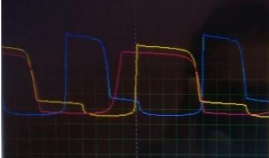
\includegraphics[height=0.2\textheight]{Figures/g2.png}}
\\
Generated PWM signal
\\
{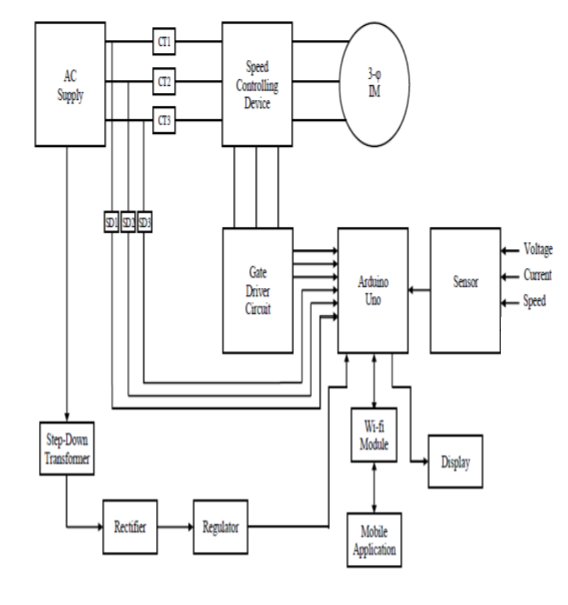
\includegraphics[height=0.4\textheight]{Figures/g3.png}}
\\
The above block diagram shows the detailed view of the project. It describes the whole project in one single diagram.
\\ \\
{\large Simulation}
\\ \\
{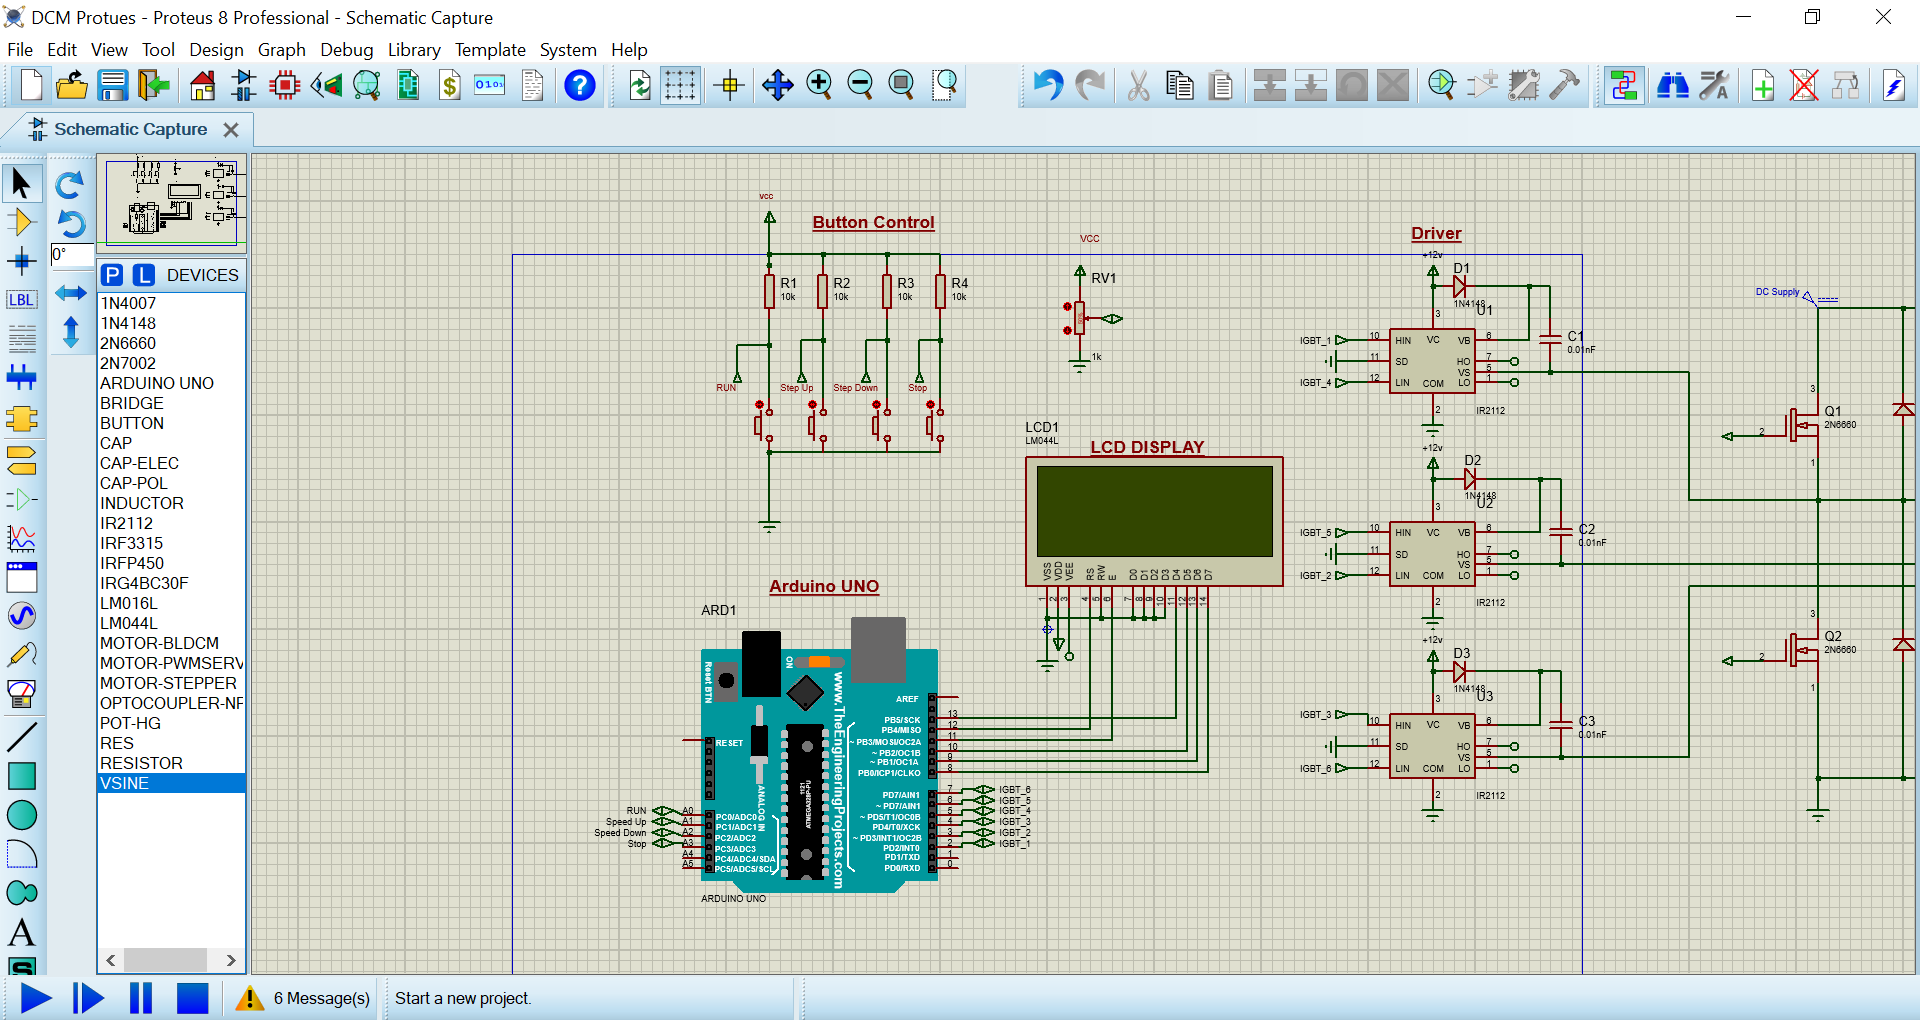
\includegraphics[height=0.3\textheight]{Figures/pro1.png}}
\\
{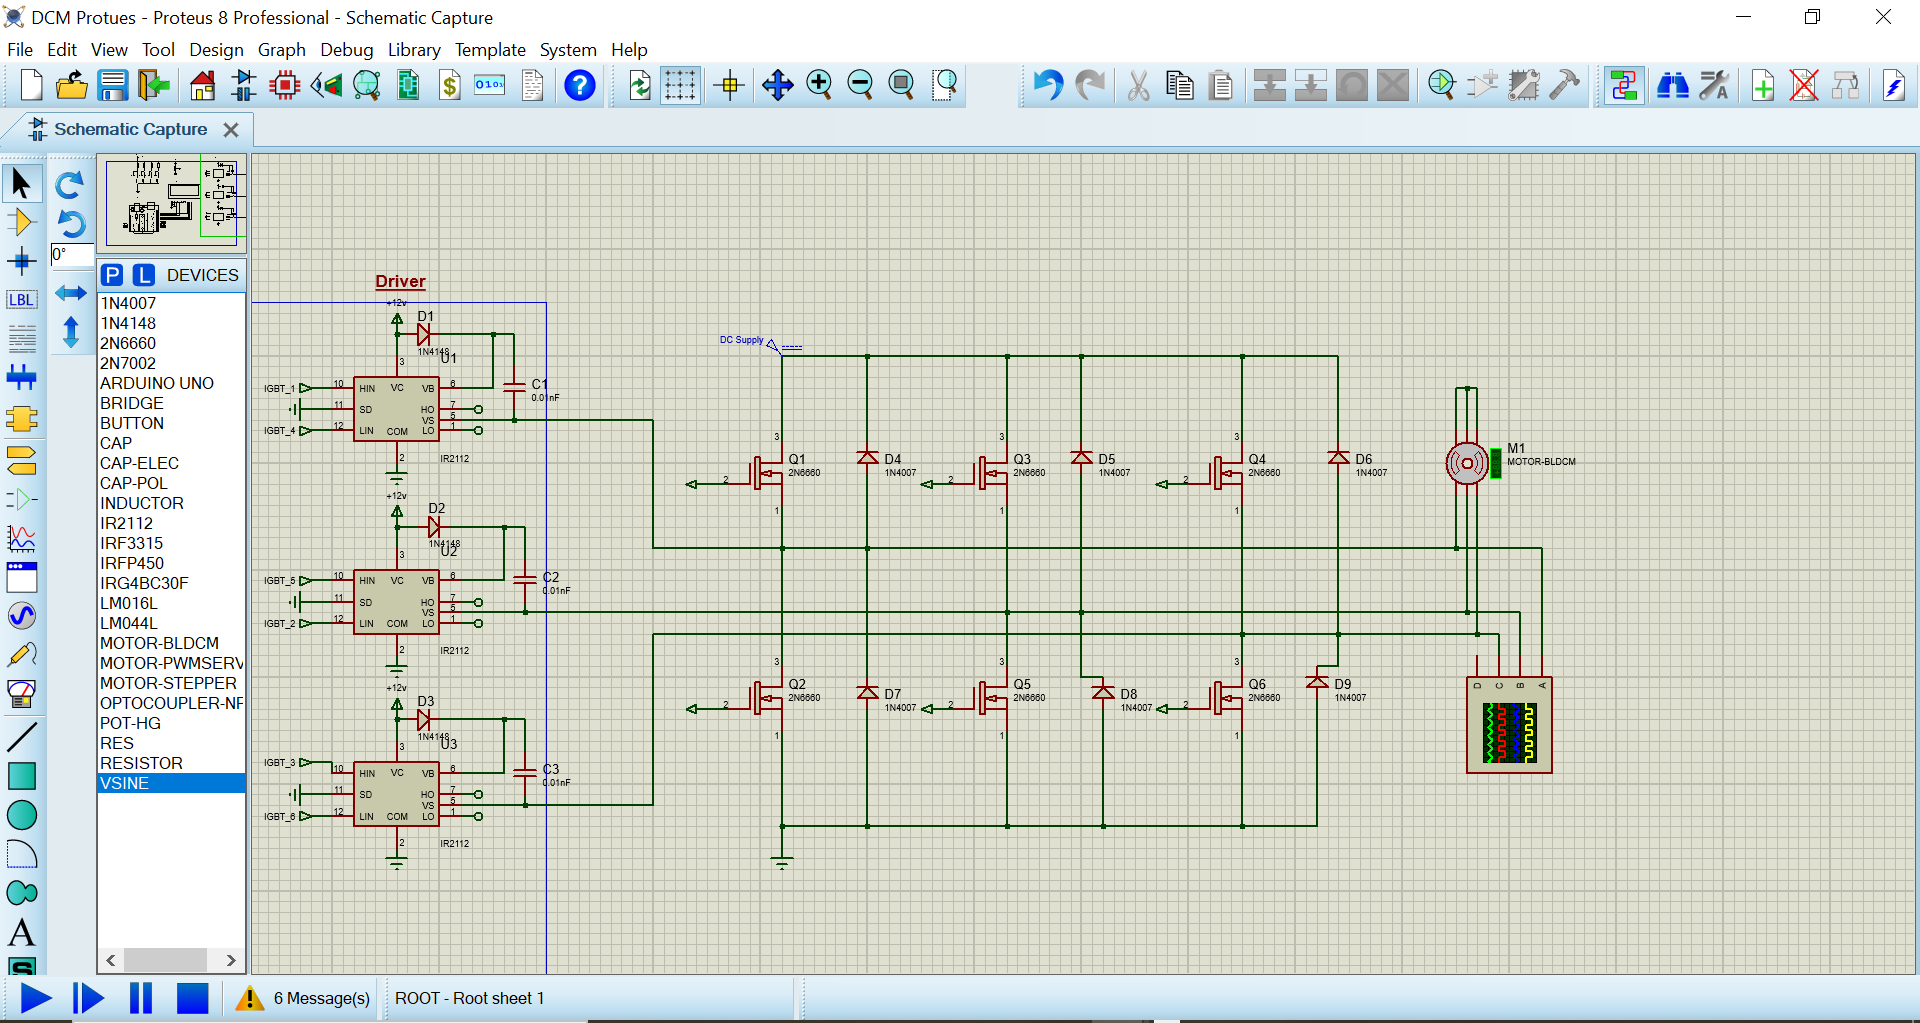
\includegraphics[height=0.3\textheight]{Figures/pro2.png}}
\\ \\






